\documentclass[runningheads]{article}
%
\usepackage[portuguese]{babel}
\usepackage[utf8]{inputenc}
\usepackage[T1]{fontenc}
\usepackage{graphicx}
\usepackage{float}
\usepackage{subfig}
\usepackage{indentfirst}
%
\usepackage{graphicx}
\usepackage{minted}


\usepackage{hyperref}
% \renewcommand\UrlFont{\color{blue}\rmfamily}
\usepackage{dirtytalk}

\begin{document}

\begin{titlepage}
\begin{center}


\includegraphics[width=0.6\textwidth]{images/EElogo.jpg}\\[0.5cm]

{\large Universidade do Minho - Escola de Engenharia}\\[0.5cm]

{\large Mestrado Integrado em Engenharia Informática}\\[0.5cm]

{\large Computação Natural}\\[0.5cm]

\vspace{2.5cm}

{ \huge \bfseries Trabalho prático \par 
Reinforcement Learning por Agentes\\[0.4cm]}

\vspace{2cm}

Carlos José Gomes Campos a74745 \\
José Pedro Ferreira Oliveira a78806 \\
Vitor José Ribeiro Castro a77870 \\

\vspace{3cm}

{\large \today}

\end{center}
\end{titlepage}

\begin{abstract}
Este relatório descreve os passos necessários ao desenvolvimento do projeto proposto pela equipa docente, a saber, a aprendizagem por reinforcement learning de um agente. O processo compreende o desenvolvimento de um modelo de reinforcement learning, - no caso, Q-Learning, - bem como a otimização dos parâmetros de treino, - no caso, através de Particle Swarm Optimization. Para tal, o ambiente de desenvolvimento requerido é Python.
Este projeto foi desenvolvido no âmbito da unidade curricular de Computação Natural, do perfil de Sistemas Inteligentes, do Mestrado Integrado em Engenharia Informática, na Universidade do Minho.

\end{abstract}

\newpage

\tableofcontents

\newpage

\section{Introdução}

\subsection{Contextualização}
\par Recentemente, com o desenvolvimento da área de \textit{machine learning} e a perceção das limitações que os paradigmas de aprendizagem supervisionada e não supervisionada têm, começou a ser dada maior importância e aplicação a \textit{reinforcement learning}.
\par Atualmente, os sistemas de informação e interação são cada vez mais dinâmicos, com mais interações a surgirem a cada momento. Com isto, os algoritmos de reinforcement learning ganham vantagem perante os outros, uma vez que permitir equilibrar a razão entre exploração de conhecimento e uso do mesmo. Adicionalmente, permite implementar ambientes formulados por um Processo de Decisão de Markov, sem ter a carga computacional necessária para a criação de um modelo grande.
\par Indubitavelmente, com o crescimento dos jogos virtuais e da necessidade de melhorar as suas ações e realidade, a inteligência artificial tem sido aplicada em cada vez mais títulos, pelo que se torna interessante explorar estes recursos.

\subsection{Caso de Estudo}
\par No caso do projeto, pretende-se aplicar a inteligência artificial numa ótica de resolução de problema, ou seja, criar um jogador inteligente. O jogo a tratar é o Pac-Man, título antigo e que, assim, permitirá a máquinas mais modestas criar agentes inteligentes que, por conceção, seriam utilizáveis em situações de maior complexidade.
\par O agente deverá ser treinado para ter a melhor \textit{performance} possível, para um mapa específico.

\subsection{Estrutura do Relatório}
\par O relatório está dividido em cinco partes, correspondentes às etapas de criação do modelo de Q-Learning, Otimização com PSO, Análise de Resultados, Análise em Outros Mapas e Conclusão.
\par Na secção \ref{QL} explica-se o processo de criação do modelo e explica-se cada umas das funções editadas, de acordo com o sugerido. Na secção \ref{PSO} descreve-se todo o algoritmo de otimização, bem como o porquê do uso desta ao invés de outas opções. Na secção \ref{AR}, faz-se a análise dos resultados obtidos ao longo das iterações de melhoramento do algoritmo de otimização. Na secção \ref{AOM}, discutem-se os desafios e melhoramentos possíveis para mapas de maior dimensão, comparando-se os resultados obtidos num mapa de tamanho médio com um mapa de tamanho pequeno.
\par O relatório termina com as conclusões na secção \ref{Conc} onde é feita uma reflexão acerca do trabalho realizado e as dificuldades sentidas ao longo do mesmo.

\newpage
\section{Modelo Q-Learning}
\label{QL} Tal como proposto no enunciado do trabalho, o grupo desenvolveu uma implementação do modelo Q-Learning para a resolução do problema, que consiste em treinar um agente para jogar Pac-Man. Esta implementação está restringida pelos módulos que dão suporte ao jogo, disponibilizados pela equipa docente. Desta forma, editou-se apenas as funções: \textit{computeValueFromQValues}, \textit{computeActionFromQValues}, \textit{getQValue}, \textit{getAction} e \textit{update}.

\subsection{\textit{computeValueFromQValues}}
Nesta função o objetivo é devolver o maior Q-Value cuja ação seja permitida. Nesse sentido, cria-se uma estrutura que reserve todos os elementos de Q-Value associados a ações legais, sendo que no fim se retorna o maior desses valores registados. Caso nenhuma ação legal exista é retornado o valor 0.0, graças às propriedades de inicialização desta estrutura.

\begin{minted}{python}
def computeValueFromQValues(self, state):
        """
          Returns max_action Q(state,action)
          where the max is over legal actions.
          Note that if there are no legal actions,
          which is the case at the terminal state,
          you should return a value of 0.0.
        """
        "*** YOUR CODE HERE ***"
        # to store legal values to iterate
        legalValues = util.Counter()
        for action in self.getLegalActions(state):
            legalValues[action] = self.getQValue(state,action)
        # return the biggest value of all
        return legalValues[legalValues.argMax()]
\end{minted}

\newpage
\subsection{\textit{computeActionFromQValues}}
Nesta função o objetivo é devolver a ação cujo \textit{Q-Value} é o maior, em relação ao conjunto de ações permitidas. É verificada a existência de ações legais e, caso não existam, é retornado um \textit{None}. Caso exista, cria-se uma estrutura que reserve todos os elementos de \textit{Q-Value} associados a ações legais, sendo que no fim se retorna a chave correspondente ao maior \textit{Q-Value} desses valores registados.

\begin{minted}{python}
def computeActionFromQValues(self, state):
        """
          Compute the best action to take in a state.
          Note that if there are no legal actions,
          which is the case at the terminal state,
          you should return None.
        """
        "*** YOUR CODE HERE ***"
        # check if there's any legal actions
        # (not in terminal state)
        actions = self.getLegalActions(state)
        if not actions:
            return None

        # to store legal values to iterate
        legalValues = util.Counter()
        for action in actions:
            legalValues[action] = self.getQValue(state,action)
        # return the key which has the biggest value
        return legalValues.argMax()
\end{minted}

\subsection{\textit{getQValue}}
Nesta função o objetivo é devolver o \textit{Q-Value} correspondente a um par \textit{State-Action}. Novamente, devido às propriedades da estrutura utilizada, é possível devolver o valor 0.0 caso um par ainda não tenha sido visitado, ou o valor respetivo caso já tenha. Para que este uso seja possível, na função \textbf{\_\_init\_\_} é inicializada a estrutura que regista os \textit{Q-Values}.

\begin{minted}{python}
def getQValue(self, state, action):
        """
          Returns Q(state,action)
          Should return 0.0 if we have never seen a state
          or the Q node value otherwise
        """
        "*** YOUR CODE HERE ***"
        return self.Qvalues[(state,action)]
\end{minted}

\subsection{\textit{getAction}}
Nesta função o objetivo é devolver a ação a tomar no estado atual. Para isso, e tendo em conta a necessidade de exploração definida em \textit{epsilon}, recorre-se à função \textbf{flipCoin} disponibilizada para ter em conta essa aleatoriedade. Num caso, opta-se por escolher de forma aleatória qualquer uma ação legal e, no outro, a ação preferível de acordo com a política existente. É verificada, naturalmente, a existência de ações legais, de modo a prever a localização em estado final.

\begin{minted}{python}
def getAction(self, state):
        """
          Compute the action to take in the current state.  With
          probability self.epsilon, we should take a random action and
          take the best policy action otherwise.  Note that if there are
          no legal actions, which is the case at the terminal state, you
          should choose None as the action.

          HINT: You might want to use util.flipCoin(prob)
          HINT: To pick randomly from a list, use random.choice(list)
        """
        # Pick Action
        legalActions = self.getLegalActions(state)
        action = None
        "*** YOUR CODE HERE ***"
        if legalActions:
            if util.flipCoin(self.epsilon):
                action = random.choice(legalActions)
            else:
                action = self.computeActionFromQValues(state)

        return action
\end{minted}

\newpage
\subsection{\textit{update}}
Esta função é disponibilizada ao motor do jogo e será chamada para atualizar os \textit{Q-Values} dos estados anteriores, após recompensa recebida. É feito o cálculo da recompensa estimada e adicionada ao \textit{Q-Value} correspondente, mediante os valores \textit{alpha} e \textit{gamma} usados na inicialização do processo de treino.

\begin{minted}{python}
def update(self, state, action, nextState, reward):
        """
          The parent class calls this to observe a
          state = action => nextState and reward transition.
          You should do your Q-Value update here

          NOTE: You should never call this function,
          it will be called on your behalf
        """
        "*** YOUR CODE HERE ***"
        estimatedQ =
            reward
            + self.discount * self.computeValueFromQValues(nextState)
        self.Qvalues[(state,action)] =
            (1 - self.alpha) * self.getQValue(state,action)
            + self.alpha * estimatedQ
\end{minted}

\newpage
\section{Otimização por PSO}
\label{PSO}
Com vista à otimização dos parâmetros a utilizar para a fase de treino do \textit{Q-Learning}, implementou-se um algoritmo de \textit{Particle Swarm Optimization}. O objetivo é que cada partícula procure os melhores valores para \textit{epsilon}, \textit{gamma} e \textit{alpha}, na medida em que um bom treino irá permitir um bom \textit{score} médio no teste do conhecimento adquirido. Cada partícula partilhará, posteriormente, o resultado do uso dos seus valores para estes parâmetros, ocorrendo um ajuste para aquele que é o melhor resultado pessoal e da população.
\par Para a realização da otimização exigida, criou-se um módulo Python de nome "pso". Este pode ser corrido com recurso ao comando \textbf{python pso.py} e implementa o algoritmo de PSO para 3 dimensões, a saber, de \textit{epsilon}, \textit{alpha} e \textit{gamma}. Adicionalmente, é também inicializado um limite para os valores que estes parâmetros a otimizar podem tomar, que é de 0 a 1 para todos.
\par O número de partículas definidas para a otimização é de 15 e o número de iterações a fazer é 30. Estes valores foram aceites como necessários e suficientes pelo grupo, tendo em conta o tempo e complexidade do problema. Para o caso em questão, o algoritmo de otimização corre em cerca de 6 horas, um valor que permite a sua execução em períodos noturnos numa máquina de 2 cores sem gpu.

\subsection{Partícula}

\par No caso em questão, uma partícula não passa de um momento de treino e teste único, que podia ser executado através do comando
\linebreak 
\textbf{python pacman.py -p PacmanQAgent -x 2000 -n 2010 -l smallGrid \linebreak -a epsilon=0.1,alpha=0.3,gamma=0.7}, para o caso em que epsilon=0.1, alpha=0.3 e gamma=0.7.
 

\par Primeiramente, é necessário inicializar o conjunto de todas as partículas. Na sua inicialização, as partículas são compostas por:
\begin{itemize}
    \item posição atual (position\_i)
    \item velocidade atual (velocity\_i)
    \item posição que melhor \textit{score} obteve (pos\_best\_i)
    \item melhor \textit{score} obtido (score\_best\_i)
    \item \textit{score} obtido na posição atual (score\_i)
\end{itemize}
\par O melhor \textit{score} é inicializado com um valor indicativo, -1, para que se saiba que ainda não foi feita qualquer avaliação até ao momento. A posição é escolhida de forma aleatória, com recurso à função random() do módulo random, que retorna um valor entre 0 e 1. Adicionalmente, a velocidade inicial é definida como sendo 0, por forma a prevenir explosão de partículas e \textit{clamping} posterior.

\subsection{Algoritmo}
\par Apesar de o algoritmo \textit{PSO} ser algo já conhecido, interessa explicar a sua aplicação no caso em específico. Assim, os passos executados são os seguintes:
\begin{itemize}
    \item Avaliar a performance da partícula, com os parâmetros atuais (posições);
    \item Verificar se a partícula obteve um resultado melhor que todos os outros que obteve anteriormente. Se sim, atualizar melhor \textit{score} e posição pessoal;
    \item Fazer a mesma verificação em relação aos resultados globais;
    \item Avaliar as partículas restantes;
    \item Recalcular as posições e velocidades das partículas;
    \item Iterar novamente por todas as partículas.
\end{itemize}

\subsection{Alternativas a PSO}
Apesar de PSO ser o algoritmo proposto no enunciado, o grupo decidiu pesquisar sobre quais as alternativas disponíveis ao uso deste. A primeira alternativa que surgiu foram Algoritmos Genéticos, devido à experiência anterior dos elementos do grupo. Esta opção foi abandonada pois percebeu-se que os GA são melhores em problemas de otimização discreta. De facto, proceder a mutações para os valores de \textit{epsilon}, \textit{alpha} e \textit{gamma} dificilmente iria levar a uma aproximação de um valor globalmente bom. O problema em questão é, reconhecidamente, de otimização contínua.
\par Partindo para o \textit{Gradient Descent}, o grupo verificou que o problema em causa não tem uma função de custo expressa e que seja derivável facilmente. De facto, não se procura a aproximação a um conjunto de pontos mas apenas a melhora de um \textit{score} cujo mínimo e máximo é desconhecido e o valor é apenas obtido no fim do cálculo, em cada partícula.
\par Analisando sob a perspetiva de Evolução Diferencial, pode-se verificar a existência de \textit{crossover} e \textit{mutation}, caindo no mesmo mal de que os Algoritmos Genéticos sofrem, ou seja, que as mutações causem mais dispersão dos resultados e sejam feitos cálculos desnecessários.
\par Adicionalmente, analisou-se o \textit{Firefly Algorithm} que, apesar de interessante, iria levar à necessidade de muitas partículas. Este algoritmo é diferenciado do PSO por conseguir encontrar vários mínimos locais e, dentro desses, encontrar o mínimo global. Se em alguns problemas isto pode ser relevante, no problema em causa não o é e iria causar mais carga computacional para um problema de relativamente pouca complexidade.
\par Por fim, tendo-se analisado outros algoritmos de forma menos aprofundada, foi possível verificar que o PSO é um algoritmo de fácil implementação e complexidade computacional baixa face a outros. Assim, faz sentido usá-lo sobre qualquer outro algoritmo analisado.

\newpage
\section{Análise de Resultados}
\label{AR}
Tendo sido corrido o algoritmo de otimização, numa primeira fase, obtiveram-se os seguintes valores que se pensavam ser ideais:
\begin{itemize}
    \item \textit{epsilon:} 0
    \item \textit{alpha:} 0.9954457084902311
    \item \textit{gamma:} 1
\end{itemize}

\par Com estes valores, o \textit{score} médio, obtido em 10 jogos, foi de 503 pontos. Este \textit{score} representa uma taxa de vitória de 100 por cento, numa série de jogos perfeitos cujo \textit{score} máximo é precisamente 503. Com estes valores de treino foram realizados mais testes que resultaram sempre numa taxa de vitória de 100 por cento.
\par Interessa também verificar o custo do processo de otimização, nesta fase inicial, que durava 7h30m, com 2 \textit{cores} de \textit{CPU}. Este valor podia ser reduzido, quer por menor número de partículas (preferencialmente), quer por menos número de iterações. Todavia, o grupo considerou este ser um tempo de execução satisfatório face à complexidade do problema.
\par No entanto, depois do estudo que o grupo decidiu fazer em relação ao comportamentodo algoritmo em outros mapas, verificou-se que havia uma importante melhora a fazer. De facto, num momento inicial do treino, acontecia frequentemente de o agente avançar para uma casa e retornar para a anterior, consecutivamente, graças à existência de todos os Q-Value ser de 0. Como é feita uma iteração sobre os Q-Value, o algoritmo selecionava sempre a primeira ação legal, apenas não o fazendo por responsabilidade de \textit{epsilon}. Assim, o grupo implementou aleatoriedade na escolha da próxima ação quando se verificasse que a escolha seria entre ações com Q-Value = 0. Com isto, verificou-se a um melhoramento na fase inicial de exploração por parte do agente, levando a duas situações: primeiramente, porque permitia explorar mais o mapa e atualizar mais rapidamente os Q-Value, tornando o treino mais eficaz; adicionalmente, reduziu o tempo de término de uma iteração de treino, pois o agente não ficaria num determinado local até que um fantasma o encontrasse.
\par Com os melhoramentos referidos, foi possível reduzir o tempo de execução da otimização. Adicionalmente, o grupo removeu a opção gráfica para os jogos de teste, o que levou a uma nova redução de tempo de execução do algoritmo, o que permitiu aumentar o número de jogos de teste, de 10 para 100. Este aumento permite remover um fator de sorte que possa ocorrer, fornecendo mais fiabilidade à escolha da melhor partícula. O número de partículas, 15, foi considerado ajustado ao problema pois reflete a norma de que o número de partículas deve ser 3 a 4 vezes superior à complexidade do problema, ou seja, de 3, sendo no caso usado um fator 5. O número de jogos de treino, 2000, não foi alterado, pois considera-se que se era suficiente para o treino anteriormente, neste momento também será. O número de iterações, 30, manteve-se após se verificar que as partículas convergem para aquela que fornece o melhor resultado. Quer os valores a otimizar, quer o estado das partículas, são apresentados de seguida, provando a sua convergência e valores finais de otimização.
\par Parâmetros finais de otimização:
\begin{itemize}
    \item \textit{epsilon:} 0
    \item \textit{alpha:} 0.8528980101257206
    \item \textit{gamma:} 1
\end{itemize}
\par Posições das partículas, atestando convergência:
\begin{itemize}
    \item \textit{epsilon:} 0, \textit{alpha:} 0.7745934340590099, \textit{gamma:} 1
    \item \textit{epsilon:} 0, \textit{alpha:} 0.534612646535806, \textit{gamma:} 1
    \item \textit{epsilon:} 0.0016595236545817545, \textit{alpha:} 0.8836159246652415, \textit{gamma:} 1
    \item \textit{epsilon:} 0, \textit{alpha:} 0.2627160232887614, \textit{gamma:} 1
    \item \textit{epsilon:} 0.0434282134806337, \textit{alpha:} 0.009128751802415236, \textit{gamma:} 1
    \item \textit{epsilon:} 0, \textit{alpha:} 0.9097169552417116, \textit{gamma:} 0.9794275617910148
    \item \textit{epsilon:} 0, \textit{alpha:} 0.7313054982529023, \textit{gamma:} 0.9946388022651523
    \item \textit{epsilon:} 0, \textit{alpha:} 0.8403468352268277, \textit{gamma:} 0.9980439869090084
    \item \textit{epsilon:} 0, \textit{alpha:} 0, \textit{gamma:} 1
    \item \textit{epsilon:} 0, \textit{alpha:} 0.5274948929730368, \textit{gamma:} 0.9998735237834728
    \item \textit{epsilon:} 0, \textit{alpha:} 0.8458936899803827, \textit{gamma:} 1
    \item \textit{epsilon:} 0, \textit{alpha:} 0.7967045785631481, \textit{gamma:} 1
    \item \textit{epsilon:} 0, \textit{alpha:} 0.8428498053783146, \textit{gamma:} 0.9923536972082919
    \item \textit{epsilon:} 0.007927716406400893, \textit{alpha:} 1, \textit{gamma:} 1
    \item \textit{epsilon:} 0.00017285003848879657, \textit{alpha:} 0.28801790569619623, \textit{gamma:} 0.9952562189914202
\end{itemize}

\newpage
\section{Análise em Outros Mapas}
\label{AOM}
Analisando a execução do algoritmo para vários mapas, foi possível tirar algumas conclusões face à eficácia e funcionamento do método. Foi possível identificar, primeiramente, que o tempo que demorava a fase de treino numa situação inicial, em que os Q-Value eram todos 0, era demasiado alta. Para corrigir isso, introduziu-se a aleatoriedade referida na secção anterior. Assim, na tabela que se mostra em baixo, é possível verificar a evolução do \textit{winrate}, em percentagem, após essas modificações.
\par Adicionalmente, e como representado pela tabela seguinte, que é relativa ao mapa \textit{mediumgrid}, desde logo é possível verificar que o número jogos de treino necessários tem que aumentar consideravelmente. Como referência, no caso da \textit{smallgrid}, que serve de base para o relatório, 2000 jogos de treino são suficientes para atingir \textit{winrates} superiores a 90 por cento dos jogos. Por oposição, 2000 jogos são indubitavelmente insuficientes quando comparamos com mapas maiores, como o \textit{mediumgrid}. De facto, só acima de 15000 jogos é que se atingem margens de vitória próximas do anterior. Isto resulta da necessidade que existe de viver todos os casos possíveis por parte do agente, por forma a registar os Q-Value de forma correta na representação do mapa. Se o tamanho do mapa aumenta de, por exemplo, 4x4, para algo como 8x8, a necessidade de iterações não duplica, pois o número de combinações possíveis de Estado-Ação cresce de forma quase exponencial.
\par Visivelmente, o número de Estado-Ação cresce de forma exponencial, levando a um consumo cada vez maior de memória e da necessidade de controlar e calcular os Q-Values novos, trazendo limitações à aplicação deste algoritmo para mapas maiores. Uma medida que pode ser útil para prevenir esta situação é reduzir o tempo inicial de aprendizagem, sendo que a forma mais fácil de o fazer é, de forma simplista, fazer manualmente alguns jogos. Esta ação permitiria mostrar ao agente uma rota de sucesso possível e que poderia ser seguida, dando claro oportunidade a alguma variância e nova aprendizagem por causa de \textit{epsilon}. Todavia, esta aproximação pode, em alguma situações, introduzir um \textit{bias} negativo à aprendizagem de soluções novas por parte do algoritmo. Outra das ações, que foi tomada pela equipa, é introduzir alguma aleatoriedade aquando da existência de valores de Q-Value iguais a 0, que podia ser extendida para quando estes valores são baixos, ou seja, próximos de 0. A título de exemplo, os primeiros jogos num mapa pequeno, \textit{smallgrid}, podiam demorar cerca de 3 segundos, ao passo que no \textit{mediumgrid} podiam demorar 7 segundos. Para um mapa maior, seria perfeitamente possível durar até minutos, pois a única maneira de o jogo acabar quando o agente não toma ações aleatórias é perder por ser atingido por um fantasma. Por fim, uma das outras possíveis atualizações a fazer ao algoritmo seria o de promover uma atualização dos Q-Value em série, ou seja, que não implicasse apenas o estado atual e o anterior, mas sim um conjunto de estados anteriores, em proporção.
\par Apresenta-se, então, a tabela de resultados, que expõe a \textit{winrate} do algoritmo para diferentes valores de \textit{epsilon}, \textit{gamma} e \textit{alpha}, que foram sendo introduzidos manualmente e numa perspetiva de exploração por parte do grupo.

\begin{figure}[H]
\centering
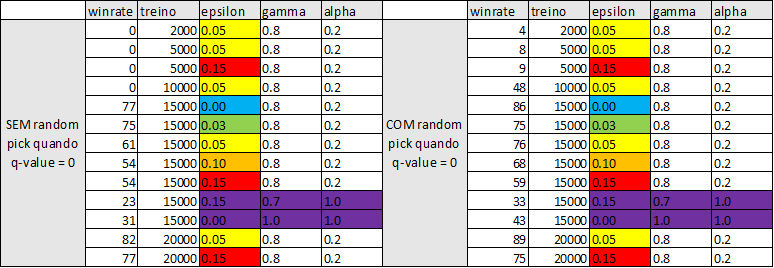
\includegraphics[width=13cm]{images/winrates.png}
\caption{\textit{winrate} por algoritmo e parâmetros, em \textit{mediumgrid}}
\end{figure}

\newpage
\section{Conclusão}
\label{Conc}
No decurso deste trabalho, o grupo encontrou algumas dificuldades e conseguiu resolver as mesmas. Se, inicialmente, a implementação do algoritmo de \textit{Q-Learning} era algo que nunca havíamos feito, depois de análise tornou-se óbvio que a dificuldade maior seria compreender os módulos fornecidos pela equipa docente.
\par Resolvida essa questão, a equipa voltou-se para a otimização dos parâmetros que já tinham um valor \textit{default}, conforme sugerido pelos criadores do exercício. O desenvolvimento e implementação do algoritmo de \textit{PSO} permitiu à equipa compreender melhor o funcionamento do mesmo e quais as vantagens face a outros algoritmos de otimização já utilizados. Foi necessário adaptar os módulos fornecidos para correr o algoritmo mas o grupo obteve os resultados que pretendia. Após a análise feita para mapas maiores, foram encontrados alguns pontos a melhorar, sendo que o grupo se sente confiante com os resultados obtidos na conclusão do trabalho.

\end{document}